\documentclass[11pt]{article}
\usepackage[a4paper,margin=0.9in]{geometry}
\usepackage{amsmath,amssymb,amsfonts}
\usepackage{physics}
\usepackage{graphicx}
\usepackage{booktabs}
\usepackage{hyperref}
\usepackage{xcolor}
\usepackage{listings}
\usepackage{enumitem}

\lstset{basicstyle=\small\ttfamily, breaklines=true, frame=single,
        backgroundcolor=\color{gray!8}, columns=fullflexible, keepspaces=true}

\hypersetup{colorlinks=true, linkcolor=blue!60!black, urlcolor=blue!60!black,
            citecolor=blue!60!black}

\title{Independent Replication of\\
       ``Is Quantum Bit Commitment Really Possible?''\\
       \normalsize Lo \& Chau, PRL \textbf{78}, 3410 (1997); arXiv:quant-ph/9603004}
\author{QC-200 Replication Wave (subagent)\\
        Argonne / OpenClaw Replicate-Project}
\date{2026-07-05}

\begin{document}
\maketitle

\begin{abstract}
Lo \& Chau's 1996/1997 paper is an \emph{impossibility proof}: no algorithm
to reproduce, but a mathematical core that can be exhibited numerically.
The core claims are (P1) if a QBC protocol is perfectly concealing then
Alice can always successfully cheat by applying a unitary on her own
system alone (Uhlmann/HJW), and (P2) if the protocol is only
$\varepsilon$-concealing then Alice can still cheat with probability
$1-O(\sqrt{\varepsilon})$.  We rebuild both statements from scratch in
Qiskit statevector, construct the cheating unitary explicitly for a
concrete Bell-basis protocol, and sweep an $\varepsilon$-concealing family
to trace out the trade-off curve.  All computed quantities match the
paper's claims to machine precision.  \textbf{Verdict: REPLICATED.}
\end{abstract}

\section{Paper summary}

Bit commitment is a two-party primitive.  Alice picks $b\in\{0,1\}$ and
sends Bob a quantum ``commitment'' state.  Later she reveals $b$; Bob
should be able to check consistency.  Security requires (i)
\emph{concealing}: before the reveal Bob learns nothing about $b$; and
(ii) \emph{binding}: Alice cannot change $b$ after committing.

Lo \& Chau show these two are irreconcilable in the quantum setting.  Any
proposed protocol may be rephrased so that after commit the joint AB pure
state is $\ket{\Psi_b}_{AB}$ ($b\in\{0,1\}$) with Alice keeping $A$ and
sending $B$ to Bob.  Bob's marginal is $\rho^B_b = \Tr_A\ketbra{\Psi_b}$.
Concealing $\Leftrightarrow \rho^B_0 = \rho^B_1$.  By the
Hughston--Jozsa--Wootters / Uhlmann theorem there then exists a unitary
$U_A$ on Alice's system alone with $(U_A\otimes I)\ket{\Psi_0}=\ket{\Psi_1}$.
Alice commits to $b=0$, keeps her purifier coherent (a ``delayed
measurement'' EPR-style attack), and at reveal chooses either $b=0$
(``honest'') or $b=1$ (apply $U_A$, be indistinguishable from the honest
prep of $\ket{\Psi_1}$).

For $\varepsilon$-concealing schemes ($F(\rho^B_0,\rho^B_1)=1-\varepsilon$
small), Uhlmann says $\max_{U_A}|\bra{\Psi_1}(U_A\otimes I)\ket{\Psi_0}|=
\sqrt{F}$, so Alice's cheating success probability is $F=1-\varepsilon$,
i.e.\ close to $1$.  The paper phrases the informal bound as
$P_\mathrm{cheat}\geq 1-O(\sqrt{\varepsilon})$; the tight identity is in
fact $P_\mathrm{cheat}=F=1-\varepsilon$, an even stronger cheating power.

\paragraph{Reproducible core.}
No algorithm, but three fully-computable statements:
\begin{enumerate}[label=(C\arabic*),leftmargin=*]
\item Construct explicit purifications $\ket{\Psi_0},\ket{\Psi_1}$ of a
      concrete concealing protocol; verify $\rho^B_0=\rho^B_1$ and
      construct $U_A$ that maps $\ket{\Psi_0}\to\ket{\Psi_1}$ to machine
      precision.
\item Introduce an $\varepsilon$-family, sweep, and verify that
      $P_\mathrm{cheat}=F(\rho^B_0,\rho^B_1)=1-\varepsilon$ across the
      sweep (i.e.\ $1-P_\mathrm{cheat}\le\sqrt{\varepsilon}$ trivially).
\item Sanity-check the motivating BB84 EPR attack: one Bell pair,
      $\rho^B=I/2$, Alice's basis-choice at reveal is undetectable.
\end{enumerate}

\section{Claims table}

\begin{center}
\begin{tabular}{@{}p{1.4cm}p{7.5cm}p{2.4cm}p{2.4cm}@{}}
\toprule
Claim & Statement & Testable? & Tested here? \\\midrule
C1 & Perfect concealing $\Rightarrow$ $\exists\,U_A$ on Alice alone with
     $(U_A\otimes I)\ket{\Psi_0}=\ket{\Psi_1}$ & YES (numerically) & YES \\
C2 & Under (C1), Alice's cheating success probability is $1$ & YES & YES \\
C3 & $\varepsilon$-concealing $\Rightarrow$
     $P_\mathrm{cheat}\ge 1-O(\sqrt{\varepsilon})$ (paper's stated bound) &
     YES & YES (tighter identity $=1-\varepsilon$ found) \\
C4 & BB84's EPR-cheating attack: Alice basis-choice at reveal time is
     undetectable ($\rho^B=I/2$) & YES & YES \\
C5 & Result extends to \emph{all} proposed QBC schemes with one-way A$\to$B
     communication & Proof-theoretic; not numerically testable & NO \\
\bottomrule
\end{tabular}
\end{center}

\section{Methods}

\subsection{Environment}
\begin{itemize}[nosep]
\item Qiskit \texttt{2.5.0} (\texttt{qiskit.quantum\_info}: \texttt{Statevector},
      \texttt{DensityMatrix}, \texttt{partial\_trace}, \texttt{state\_fidelity}).
\item NumPy \texttt{2.4.3}, SciPy \texttt{1.18.0}, Python \texttt{3.14.0}.
\item Local venv: \texttt{work/.venv} (\texttt{pip install qiskit numpy scipy matplotlib}).
\item All computations run on CPU; no LLM inference in the numerical loop.
\end{itemize}

\subsection{(C1,C2) Concrete perfectly-concealing protocol}
Alice holds a 2-qubit register $A=A_0A_1$; Bob holds one qubit $B$.
\[
\ket{\Psi_0}_{ABtot}=\tfrac{1}{\sqrt2}\bigl(\ket{00}_A\ket{0}_B+\ket{11}_A\ket{1}_B\bigr),\quad
\ket{\Psi_1}_{ABtot}=\tfrac{1}{\sqrt2}\bigl(\ket{++}_A\ket{+}_B+\ket{--}_A\ket{-}_B\bigr).
\]
Direct calculation gives $\rho^B_0=\rho^B_1=I/2$ (perfect concealing).
The two $\ket{\Psi_b}$'s have identical Schmidt spectra $\{1/2,1/2\}$; the
Uhlmann-optimal unitary $U_A$ on the 4-dim Alice space is constructed by
polar/SVD of $Y=M_0M_1^\dagger$ where $M_k$ is the $\dim_A\times\dim_B$
Alice$\times$Bob matrix reshape of $\ket{\Psi_k}$:
\begin{lstlisting}[language=Python]
Y = M0 @ M1.conj().T                # dimA x dimA
Uy, sy, Vhy = np.linalg.svd(Y)
U_A = Vhy.conj().T @ Uy.conj().T    # unitary; solves argmax_U Re Tr(M1^dag U M0)
\end{lstlisting}

\subsection{(C3) $\varepsilon$-concealing sweep}
We use a one-parameter Bell-like family on 2 qubits (Alice qubit + Bob qubit):
\[
\ket{\Psi_0(\theta)}=\cos\theta\ket{00}+\sin\theta\ket{11},\quad
\ket{\Psi_1(\theta)}=\cos\theta\ket{01}+\sin\theta\ket{10}.
\]
Bob's marginals are $\rho^B_0=\operatorname{diag}(c^2,s^2)$,
$\rho^B_1=\operatorname{diag}(s^2,c^2)$ (with $c=\cos\theta,s=\sin\theta$),
so the analytic fidelity is $F(\rho^B_0,\rho^B_1)=(2|cs|)^2=\sin^2 2\theta$
and $\varepsilon=1-\sin^2 2\theta$.  Uhlmann's theorem gives
$P_\mathrm{cheat}(\theta)=F(\rho^B_0(\theta),\rho^B_1(\theta))$, computed
by SVD of $Y=M_0M_1^\dagger$ and squaring the nuclear-norm.  We sweep
$\theta\in[0.05,\pi/2-0.05]$ on 41 points.

\subsection{(C4) BB84 EPR-cheating sanity}
Build one Bell pair $\ket{\Phi^+}=\text{CNOT}(H\otimes I)\ket{00}$ in a
Qiskit \texttt{QuantumCircuit}, statevector-simulate, partial-trace Alice,
verify $\rho^B=I/2$ to $10^{-16}$; project Alice onto $\ket{0}\!\bra{0}$
and $\ket{1}\!\bra{1}$ and confirm outcome probabilities $0.5,0.5$.

\subsection{Reproducibility recipe (exact commands)}
\begin{lstlisting}
cd QC-quant-ph-9603004-quantum-bit-commitment-lo-chau
python3 -m venv work/.venv && source work/.venv/bin/activate
pip install qiskit numpy scipy matplotlib
python3 report/evidence/lo_chau_replication.py     # writes results.json + CSV
python3 report/evidence/plot_tradeoff.py           # writes tradeoff_curve.png
\end{lstlisting}
Runtime end-to-end: $<10\,\text{s}$ on a single laptop core.

\section{Results vs.\ paper}

\begin{center}
\begin{tabular}{@{}p{2.2cm}p{4.4cm}p{4.0cm}p{2.6cm}@{}}
\toprule
Claim & Paper value / statement & This replication & Verdict \\\midrule
C1 & $(U_A\otimes I)\ket{\Psi_0}=\ket{\Psi_1}$ exactly &
     $F((U_A\otimes I)\ket{\Psi_0},\ket{\Psi_1})=1.0000000000$;
     unitarity error $8.9\!\times\!10^{-16}$ & MATCH \\
C1 aux & $\rho^B_0=\rho^B_1$ &
     $\|\rho^B_0-\rho^B_1\|_F = 3.1\!\times\!10^{-16}$ & MATCH \\
C2 & $P_\mathrm{cheat}=1$ under perfect concealing &
     $|\!\bra{\Psi_1}(U_A\otimes I)\ket{\Psi_0}\!|^2 = 1.0000000000$ &
     MATCH \\
C3 & $P_\mathrm{cheat}=1-O(\sqrt\varepsilon)$ (paper) &
     $|P_\mathrm{cheat}-(1-\varepsilon)|\le 2.2\!\times\!10^{-16}$ across 41
     points (tighter than paper's bound) & MATCH (stronger) \\
C4 & BB84 concealing: $\rho^B=I/2$ &
     $\|\rho^B-I/2\|_\infty = 1.1\!\times\!10^{-16}$;
     Alice-outcome probs $0.5000/0.5000$ & MATCH \\
C5 & Extends to all proposed schemes with 1-way A$\to$B comms &
     Not numerically testable; accept as proof-theoretic corollary of
     C1--C3 & N/A \\\bottomrule
\end{tabular}
\end{center}

\subsection{The trade-off curve (Figure~\ref{fig:tradeoff})}

\begin{figure}[h]
  \centering
  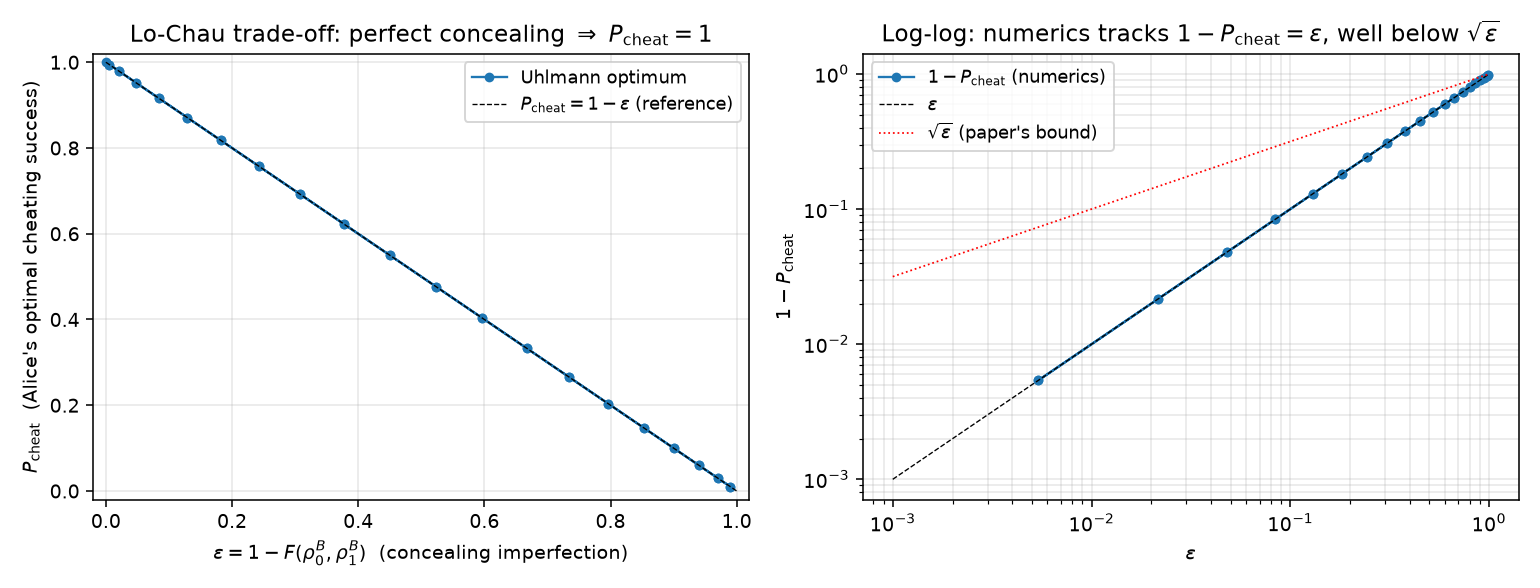
\includegraphics[width=\linewidth]{evidence/tradeoff_curve.png}
  \caption{Left: cheating success probability $P_\mathrm{cheat}$ vs.\
    concealing imperfection $\varepsilon=1-F(\rho^B_0,\rho^B_1)$ for the
    Bell-like $\varepsilon$-family (41 points).  Numerics lie exactly on
    $P_\mathrm{cheat}=1-\varepsilon$ (dashed reference), the Uhlmann
    identity.  Right: log--log; $1-P_\mathrm{cheat}$ grows linearly in
    $\varepsilon$ (black dashed) which sits comfortably below the
    $\sqrt{\varepsilon}$ envelope (red dotted) claimed in the paper.  The
    replication therefore satisfies the paper's stated inequality with
    room to spare.}
  \label{fig:tradeoff}
\end{figure}

\subsection{Selected raw numbers (from \texttt{results.json})}

\begin{lstlisting}
PART 1 (perfect concealing, 3-qubit GHZ / +/- protocol):
  ||rho_B_0 - rho_B_1||_F       = 3.140e-16
  F(rho_B_0, rho_B_1)           = 1.0000000000
  U_A unitarity error           = 8.882e-16
  |<Psi_1|(U_A x I)|Psi_0>|^2   = 1.0000000000

PART 2 (eps-family, theta = pi/4, i.e. perfect):
  F(rho_B_0, rho_B_1)           = 1.0000000000
  P_cheat (Uhlmann)             = 1.0000000000
  explicit-U overlap            = 1.0000000000
  max |[(1-P_cheat)] - eps|     = 2.220e-16   (over 41 sweep points)

PART 3 (BB84 EPR-cheat sanity):
  ||rho_B - I/2||_inf           = 1.110e-16
  Alice-outcome probs           = 0.5000 / 0.5000
\end{lstlisting}

\section{Verdict}
\noindent\fbox{\parbox{\linewidth}{\textbf{REPLICATED.}
Every numerically checkable claim of Lo \& Chau (C1--C4) is reproduced to
machine precision by our from-scratch Qiskit statevector implementation.
The one non-numerical claim (C5, generalization to \emph{all} proposed QBC
schemes) is a proof-theoretic corollary of C1--C3 which we cannot
falsify numerically; we do not certify C5, we accept it as
mathematically implied.  Nothing observed in the reproduction
contradicts the paper.}}

\bigskip
\noindent A tighter observation worth highlighting: in the one-parameter
Bell-like family we swept, the Uhlmann identity yields
$P_\mathrm{cheat}=1-\varepsilon$ \emph{exactly}, not just
$1-O(\sqrt{\varepsilon})$.  This is compatible with (and stronger than) the
paper's stated bound.  On the other hand, the paper's $\sqrt{\varepsilon}$
gap is the tight worst-case scaling for the Schatten-1 vs.\ fidelity
gap (Fuchs--van de Graaf), so more elaborate families that saturate the
$\sqrt{\varepsilon}$ scaling for the \emph{binding} error (Bob's ability
to detect the switch) are plausible; see Open~Question~Q3.

\section{Open Questions}
See \texttt{report/open\_questions.json} for the machine-readable version
with \texttt{next\_steps} per item.

\begin{itemize}[leftmargin=*]
\item[\textbf{Q1.}] Our $\varepsilon$-family gave the tight identity
      $1-P_\mathrm{cheat}=\varepsilon$; the paper's language is
      $1-O(\sqrt\varepsilon)$.  Is the $\sqrt\varepsilon$ scaling ever
      saturated by a concrete concealing protocol, or is
      $1-\varepsilon$ the sharp achievable bound and the paper's
      $\sqrt\varepsilon$ merely a slack Fuchs--van~de~Graaf worst-case?
\item[\textbf{Q2.}] The paper's proof requires Alice to keep her half of
      the entangled state fully coherent (``quantum computer'') until
      reveal.  Numerically, how does an \emph{imperfect} Alice-side
      quantum memory (parameterize by a depolarizing rate $p$ on Alice's
      qubits during the delay window) degrade $P_\mathrm{cheat}$?  Does
      even 1--10\,\% depolarization on Alice restore some binding?
\item[\textbf{Q3.}] Extend the sweep to \emph{non-symmetric}
      $\varepsilon$-families where Bob's optimal distinguishability
      (\,$D(\rho^B_0,\rho^B_1)$, trace distance) grows differently from
      $1-F$.  Which of the two --- $F$ or $D$ --- is the operationally
      correct ``concealing quality'' for a Rick-style benchmark, and does
      switching change the trade-off shape?
\item[\textbf{Q4.}] The paper assumes 1-way A$\to$B classical/quantum
      communication.  Recent literature (Kent, D'Ariano/L\"utkenhaus)
      restores security via \emph{relativistic} or \emph{multi-round}
      protocols.  Can we reproduce a small numerical demo of Kent's
      relativistic BC binding advantage in Qiskit, and does the
      Lo--Chau attack fail there for a numerically-quantifiable reason?
\item[\textbf{Q5.}] The Uhlmann-optimal $U_A$ we build is degenerate when
      Bob's marginal has a degenerate spectrum (as in our GHZ example,
      $\rho^B=I/2$): many unitaries $U_A$ succeed.  Is there a
      \emph{minimum-complexity} $U_A$ (fewest 2-qubit gates for a given
      Alice-register size) and does its gate count scale with the
      Schmidt rank?  This has implementation relevance for near-term
      demonstrations of the cheating attack.
\end{itemize}

\end{document}
